\documentclass[11pt,a4j,ascmac]{jarticle}
\usepackage{epsf}
\usepackage[dvips]{graphicx}
\usepackage{float}
\usepackage{listings}

\makeatletter
\newcommand{\subsubsubsection}{\@startsection{paragraph}{4}{\z@}%
  {1.0\Cvs \@plus.5\Cdp \@minus.2\Cdp}%
  {.1\Cvs \@plus.3\Cdp}%
  {\reset@font\sffamily\normalsize}
}
\makeatother
\setcounter{secnumdepth}{4}


\setlength{\textheight}{25cm}
\setlength{\textwidth}{16cm}
\setlength{\topmargin}{-2.5cm}
\setlength{\oddsidemargin}{0mm}
\setlength{\parindent}{0pt}
\setlength{\parskip}{3mm}

\title{第8月 進捗確認会報告資料\\
変形ARマーカの検出・推定}

\author{安井 理}
\date{令和2年10月06日}
\begin{document}
\maketitle
\section{はじめに}
\quad  キャッシュレス決済や物品管理,広告,ロボットの認識機能等の分野で QR コードや AR マーカに代表される 2 次元コードが利用されている.2 次元コードには,数百から数千バイトの情報を埋め込むことができ,シンボルと呼ばれ特殊なパターンによって視点が変化しても高精度な検出が可能である.さらに,2 次元コードの大きさを事前に定義すればカメラの位置・姿勢を推定することができる.しかし,2 次元コードは平面に貼ることを前提条件としており,曲面に貼られた 2 次元コードは歪みによる見えの変化を引き起こすため,認識精度が低下する問題を抱えている.
そこで,前任者の鈴木さんの研究では機械学習により変形した AR マーカを認識する手法を提案する.変形した画像をFasterRCNN[1] により学習することで,歪みを含む画像を正確に認識し,ID,座標,大きさ,変形度合いを推定を行った,今回行っている研究ではFasterRCNNでは座標,大きさ,変形度合いの推定が明確に行うことができないため,Augumented Autencoder[2]を用いて正確に姿勢情報を推定し,推定した情報から歪みを取り除き正面から観測した ARマーカ画像に変換する.

%------------------------------------------------------------------------------------------------------------------------------------
\section{進捗報告}
\quad 今回の進捗報告の内容を以下に示す.

\begin{itemize}

\item Tensorflow-gpuの動作確認
\item AAEのトレーニング

\end{itemize}


%-------------------------------------------------------------------------------------------------------------------------
\subsubsection{Tensorflowの概要・特徴}


\subsubsubsection{Tensorflowの概要}

\quad 機械学習の分野で使用するためのOSS(オープンソフトウェアライブラリ)であり,開発元がGoogle Brainチームである.\\
\quad 対応OS: Linux, macOS, Windows, Android, iOS... \\
\quad 対応言語:C言語,C++,Python,Java,Goなどと機械学習の分野で幅広く使用されるものである.

\  主に以下の特徴が挙げられる

\begin{description}
  \item ・データの読み込み、前処理、計算、状態、出力などを多次元的に処理する
 \item ・分散処理が可能なためビッグデータ(大量のデータ)も扱える
\end{description}


\subsubsubsection {OSS}
\  ソースコードの学習や変更・配布することが認められているライブラリ


\subsubsubsection{Tensorflow 最終環境}

\quad CUDA9.0,cuDNN7.0,Tensorflow-gpu1.12.0が現在使っているPCでTensorflow-gpuを動作させられるversionである.


\subsubsubsection{GPU確認コマンド}

\quad GPU確認コマンドで確かめた際,gpuがうまく動作したときと動作しなかったときの出力の違いを以下に示す.\\ \\


\quad GPUが動作しなかったときの出力

\begin{lstlisting}[basicstyle=\ttfamily\footnotesize, frame=single]

physical_device_desc: "device: XLA_GPU device"
   
\end{lstlisting}

\quad おそらくオンボードのGPUが反応していまっていたのではないかと考えられる.\\
\\
\\

\quad GPUが動作したときの出力

\begin{lstlisting}[basicstyle=\ttfamily\footnotesize, frame=single]

physical_device_desc: "device: 0, name: 
GeForce GTX 1080, pci bus id: 0000:01:00.0, compute capability: 6.1"

   
\end{lstlisting}

\quad deviceがGeForce GTX1080とGPUの名前に代わっており学習にGPUが使用されることも確認できた.変更点としてはCUDA9.0に対応するTensorflowのバージョンを色々試し,最終的に最新の1.12.0がうまくいった.
%--------------------------------------------------------------------------------------------------------------------










%------------------------------------------------------------------------------------------------------------------------------------
\subsubsection{AAEのおさらい}
\subsubsubsection{AAEの概要}

\quad AAEはimplicit 3d orientation learning for 6d object detection from rgb images[2] の論文で提案された手法であり,ECCV2018のBest paperに選ばれた6次元物体検出の論文である.\\
\ 6D物体検出は,3次元空間座標だけでなく3方向の向き姿勢情報も含んだ検出問題であり,高速に推定を行えることに加え,6Dのラベル付き教師データがなくても学習可能な手法である,6Dラベル付き教師データの代わりに,検出対象となる物体の3D CADデータが必要となる.全体の処理の流れ図1としては,まず入力となるRGB画像に対してSSDを用いて対象物体のBounding Boxを推定,その後,推定されたBounding Box領域から物体の姿勢情報を推定するという処理を行う,後半のBounding Box領域から物体の姿勢情報を推定する部分が今回自分の研究に取り入れようと考えている方法で,AAEという手法が用いられている.全体の流れを図\ref{fig:style1}図\ref{fig:style2}に示す.\\   
      \begin{figure}[htpp]
      \centering
      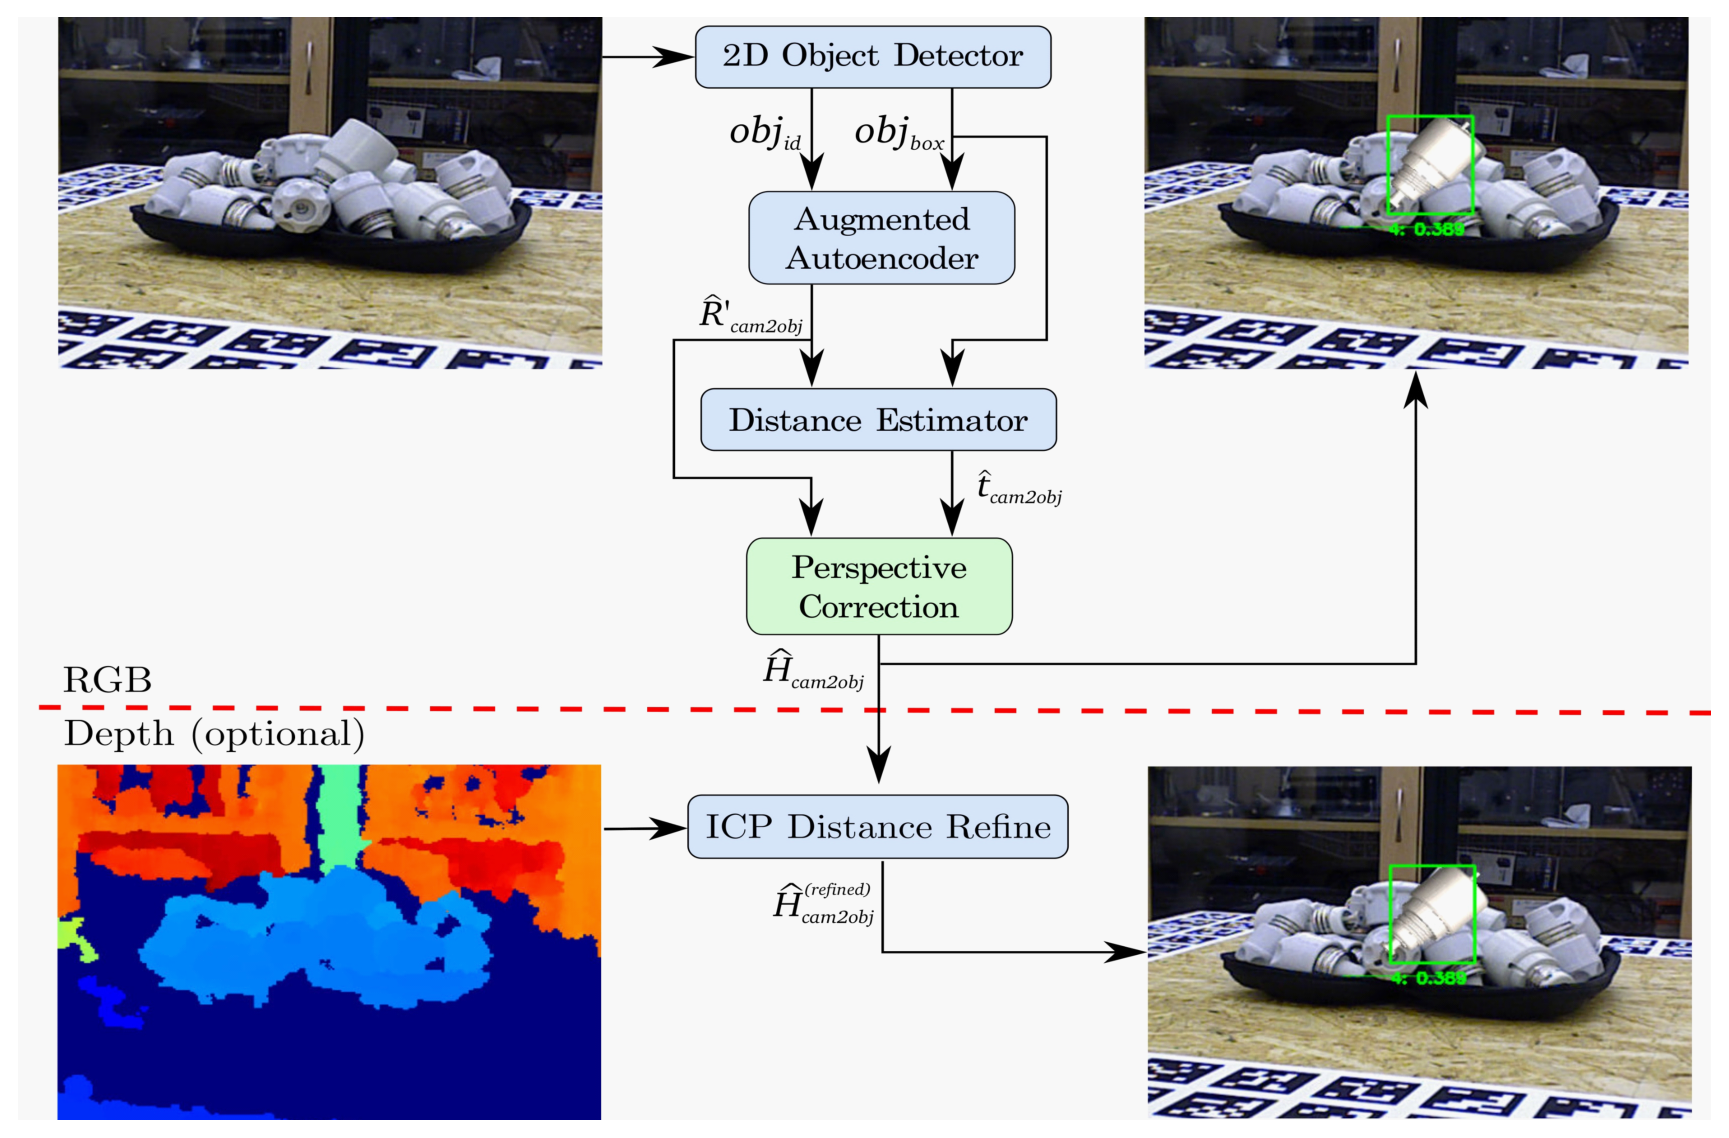
\includegraphics[width=100mm]{pic1.eps}
      \vspace*{15mm}
      \caption{全体の流れ.}
      \label{fig:style1}
      \end{figure}

      \begin{figure}[htpp]
      \centering
      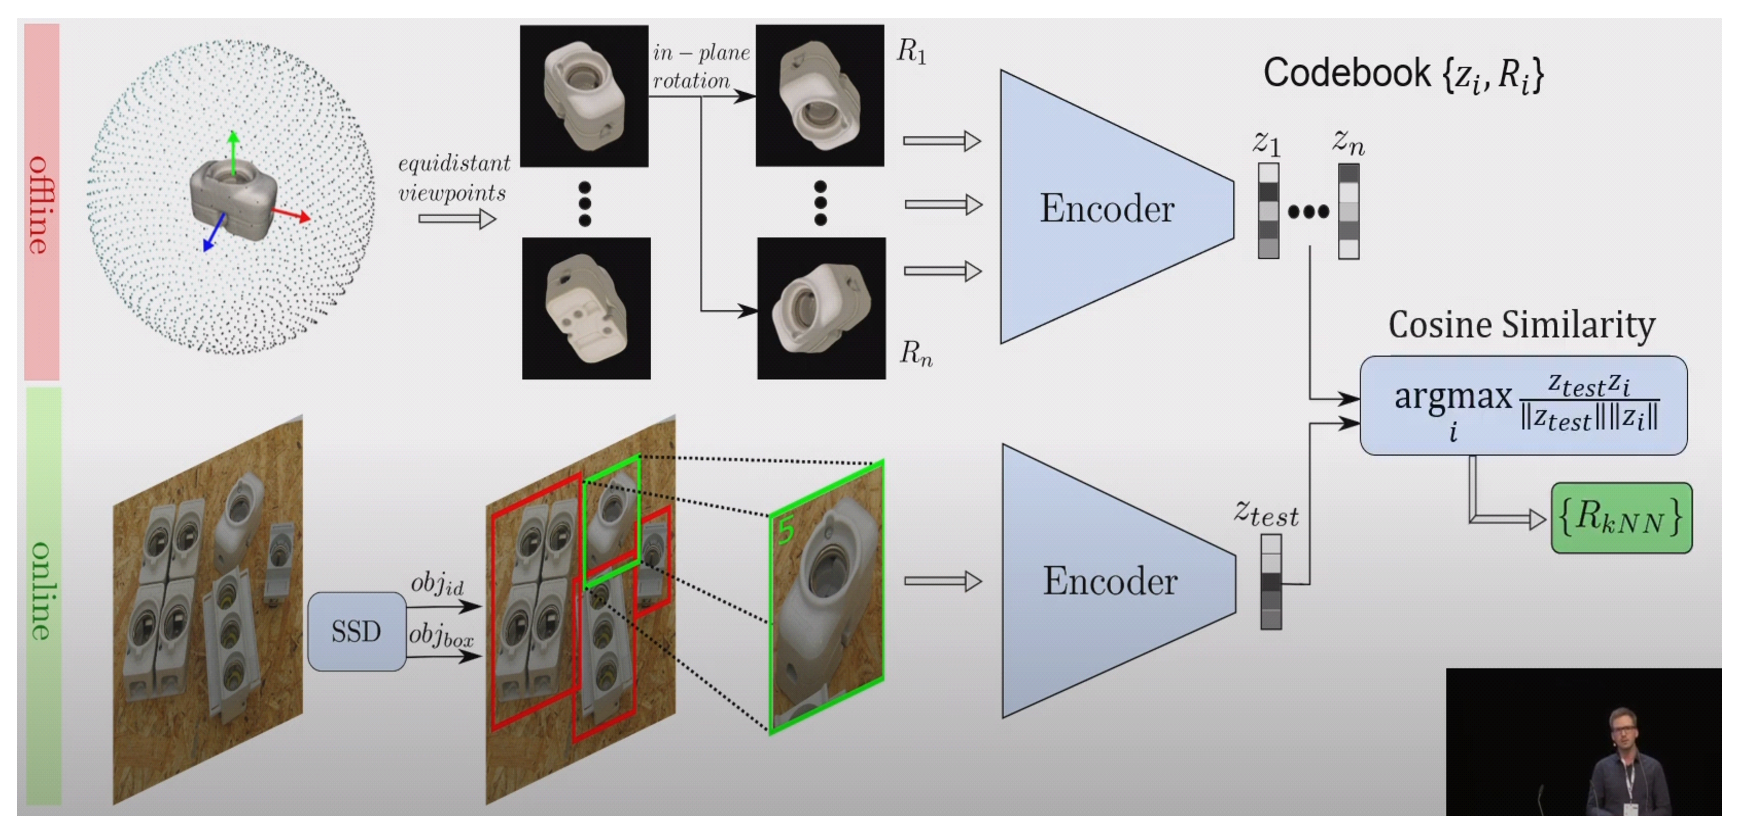
\includegraphics[width=100mm]{pic3.eps}
      \vspace*{25mm}
      \caption{全体の流れ2.}
      \label{fig:style2}
      \end{figure}



%-------------------------------------------------------------------------------------------------------------------------------------

\subsection{AAEのトレーニング}
\quad  今回はトレーニングを行う段階まで進められた.まずトレーニングは学習したい物体の様々な視点から見た画像を計92232通り用意しそれを環境画像(VOCのデータセット[3][4])に張り付けノイズを生成したものを用意する.準備した画像を図\ref{fig:style3}に示す.

\begin{figure}[htbp]
 \centering
  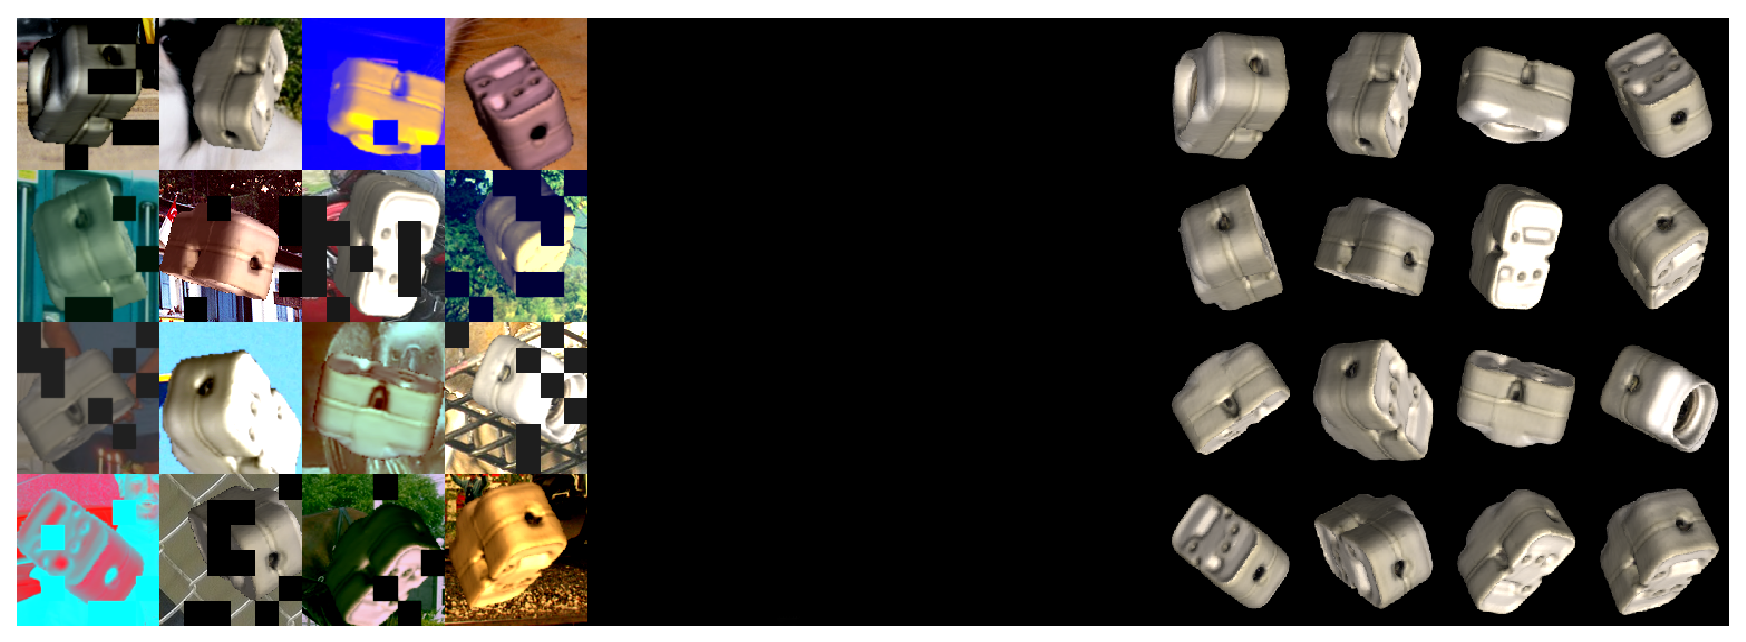
\includegraphics[width=110mm]{pic2.eps}
  \vspace*{25mm}
  \caption[図.1]{トレーニングイメージ.}
  \label{fig:style3}
\end{figure}







%-------------------------------------------------------------------------------------------------------------------


%--------------------------------------------------------------------------------------------------------------------
\section{おわりに}
\ 今回までTensorflowのバージョン合わせに時間を取られ実際の研究を進めることができず,一か月の内容としても進捗状況も進みが悪くなっていたが,やることとしては明確になっているので,ペースアップをしていきたいと思っている.これまではトレーニング部分を完了したので次にやることとしては姿勢推定を行うテスト,自分の研究のARマーカ―モデルの作成,これを用いたテスト,二次元の検出からのAAEを用いた姿勢推定までの流れを行うという順番で研究を進めていきたいと考えている.
\footnotesize
\begin{thebibliography}{99}



\bibitem{fasterrcnn}
S.Ren {\em et al. }: ``Faster R-CNN: Towards Real-Time Object Detectionwith Region Proposal Networks'', Proc. of NIPS,2015.


\bibitem{Implicit 3D Orientation Learning for 6D Object Detection from RGB Images}
Martin Sundermeyer Zoltan-Csaba Marton Maximilian Durner Rudolph Triebel , 2018 https://arxiv.org/pdf/1902.01275.pdf


\bibitem{VOC2007}
``The PASCAL Visual Object Classes Challenge 2007''.http://host.robots.ox.ac.uk/pascal/VOC/voc2007/index.html

\bibitem{VOC2012}
``Visual Object Classes Challenge 2012'',http://host.robots.ox.ac.uk/pascal/VOC/voc2012/index.html


\bibitem{VOC16}
Karen Simonyan,Andrew Zisserman,``VERY DEEP CONVOLUTIONAL NETWORKS FOR LARGE-SCALE IMAGE RECOGNITION'',2015.


\end{thebibliography}

\normalsize

\end{document}